\begin{enigme}[La dalle (d’après le GVJM)]

Dans un jardin carré de 10 m de côté, Maurice tend une corde entre chaque coin et le milieu du côté opposé, comme indiqué sur la figure. Les quatre cordes ainsi tendues délimitent une surface à l’intérieur de laquelle des ouvriers coulent une dalle en ciment (partie ombrée). Quelle est l’aire de cette dalle ? \\[0.5em]
Indice : fais pivoter certains triangles.
\begin{center} 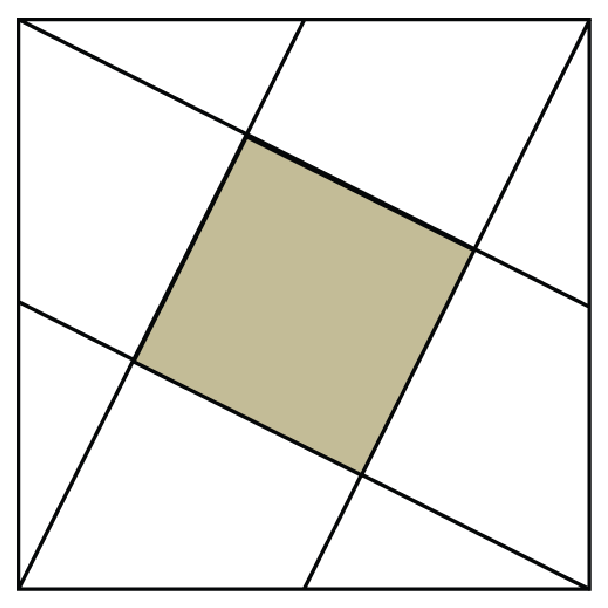
\includegraphics[width=4.7cm]{dalleGVJM} \end{center}
\end{enigme} 

%%%%%%%%%%%%%%%%%%%%%%%%%%%%%%%%%%%%%%%%%%%%%%%%%%%%%%%%%%%%%%%%%%%%%%%%%

\begin{enigme}[La disparition (d’après le GVJM)]

Construis 7 bâtonnets de 2 cm de hauteur et distants chacun de 1 cm, selon le croquis ci-dessous. Trace une ligne comme indiqué, du bas du premier bâtonnet au haut du dernier. Coupe ta figure en deux, le long de la ligne tracée. En translatant la partie du haut contre la partie du bas le long de la ligne de coupe, tu peux faire disparaître un bâtonnet. \\[0.5em]
Comment expliques-tu ce tour de magie ?
\begin{center} 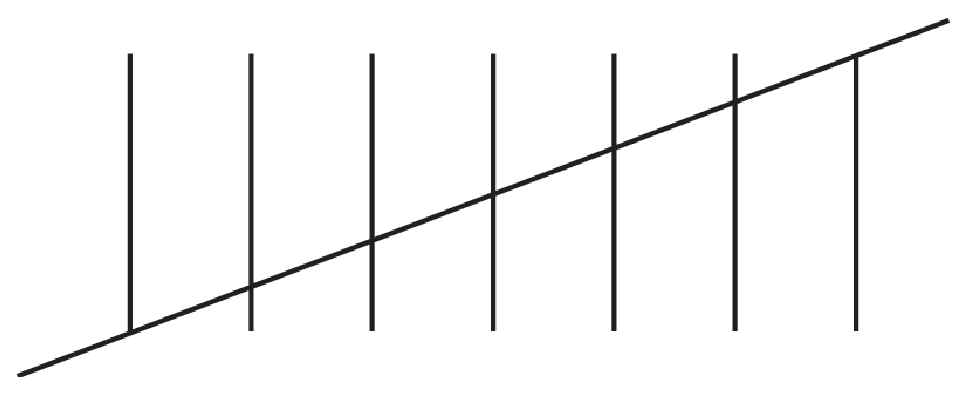
\includegraphics[width=7.5cm]{dalle_magie} \end{center}
\end{enigme} 